\documentclass[1p]{elsarticle_modified}
%\bibliographystyle{elsarticle-num}

%\usepackage[colorlinks]{hyperref}
%\usepackage{abbrmath_seonhwa} %\Abb, \Ascr, \Acal ,\Abf, \Afrak
\usepackage{amsfonts}
\usepackage{amssymb}
\usepackage{amsmath}
\usepackage{amsthm}
\usepackage{scalefnt}
\usepackage{amsbsy}
\usepackage{kotex}
\usepackage{caption}
\usepackage{subfig}
\usepackage{color}
\usepackage{graphicx}
\usepackage{xcolor} %% white, black, red, green, blue, cyan, magenta, yellow
\usepackage{float}
\usepackage{setspace}
\usepackage{hyperref}

\usepackage{tikz}
\usetikzlibrary{arrows}

\usepackage{multirow}
\usepackage{array} % fixed length table
\usepackage{hhline}

%%%%%%%%%%%%%%%%%%%%%
\makeatletter
\renewcommand*\env@matrix[1][\arraystretch]{%
	\edef\arraystretch{#1}%
	\hskip -\arraycolsep
	\let\@ifnextchar\new@ifnextchar
	\array{*\c@MaxMatrixCols c}}
\makeatother %https://tex.stackexchange.com/questions/14071/how-can-i-increase-the-line-spacing-in-a-matrix
%%%%%%%%%%%%%%%

\usepackage[normalem]{ulem}

\newcommand{\msout}[1]{\ifmmode\text{\sout{\ensuremath{#1}}}\else\sout{#1}\fi}
%SOURCE: \msout is \stkout macro in https://tex.stackexchange.com/questions/20609/strikeout-in-math-mode

\newcommand{\cancel}[1]{
	\ifmmode
	{\color{red}\msout{#1}}
	\else
	{\color{red}\sout{#1}}
	\fi
}

\newcommand{\add}[1]{
	{\color{blue}\uwave{#1}}
}

\newcommand{\replace}[2]{
	\ifmmode
	{\color{red}\msout{#1}}{\color{blue}\uwave{#2}}
	\else
	{\color{red}\sout{#1}}{\color{blue}\uwave{#2}}
	\fi
}

\newcommand{\Sol}{\mathcal{S}} %segment
\newcommand{\D}{D} %diagram
\newcommand{\A}{\mathcal{A}} %arc


%%%%%%%%%%%%%%%%%%%%%%%%%%%%%5 test

\def\sl{\operatorname{\textup{SL}}(2,\Cbb)}
\def\psl{\operatorname{\textup{PSL}}(2,\Cbb)}
\def\quan{\mkern 1mu \triangleright \mkern 1mu}

\theoremstyle{definition}
\newtheorem{thm}{Theorem}[section]
\newtheorem{prop}[thm]{Proposition}
\newtheorem{lem}[thm]{Lemma}
\newtheorem{ques}[thm]{Question}
\newtheorem{cor}[thm]{Corollary}
\newtheorem{defn}[thm]{Definition}
\newtheorem{exam}[thm]{Example}
\newtheorem{rmk}[thm]{Remark}
\newtheorem{alg}[thm]{Algorithm}

\newcommand{\I}{\sqrt{-1}}
\begin{document}

%\begin{frontmatter}
%
%\title{Boundary parabolic representations of knots up to 8 crossings}
%
%%% Group authors per affiliation:
%\author{Yunhi Cho} 
%\address{Department of Mathematics, University of Seoul, Seoul, Korea}
%\ead{yhcho@uos.ac.kr}
%
%
%\author{Seonhwa Kim} %\fnref{s_kim}}
%\address{Center for Geometry and Physics, Institute for Basic Science, Pohang, 37673, Korea}
%\ead{ryeona17@ibs.re.kr}
%
%\author{Hyuk Kim}
%\address{Department of Mathematical Sciences, Seoul National University, Seoul 08826, Korea}
%\ead{hyukkim@snu.ac.kr}
%
%\author{Seokbeom Yoon}
%\address{Department of Mathematical Sciences, Seoul National University, Seoul, 08826,  Korea}
%\ead{sbyoon15@snu.ac.kr}
%
%\begin{abstract}
%We find all boundary parabolic representation of knots up to 8 crossings.
%
%\end{abstract}
%\begin{keyword}
%    \MSC[2010] 57M25 
%\end{keyword}
%
%\end{frontmatter}

%\linenumbers
%\tableofcontents
%
\newcommand\colored[1]{\textcolor{white}{\rule[-0.35ex]{0.8em}{1.4ex}}\kern-0.8em\color{red} #1}%
%\newcommand\colored[1]{\textcolor{white}{ #1}\kern-2.17ex	\textcolor{white}{ #1}\kern-1.81ex	\textcolor{white}{ #1}\kern-2.15ex\color{red}#1	}

{\Large $\underline{12a_{0261}~(K12a_{0261})}$}

\setlength{\tabcolsep}{10pt}
\renewcommand{\arraystretch}{1.6}
\vspace{1cm}\begin{tabular}{m{100pt}>{\centering\arraybackslash}m{274pt}}
\multirow{5}{120pt}{
	\centering
	\includegraphics[width=112pt]{../../../GIT/diagram.site/Diagrams/png/1062_12a_0261.png}\\
\ \ \ A knot diagram\footnotemark}&
\allowdisplaybreaks
\textbf{Linearized knot diagam} \\
\cline{2-2}
 &
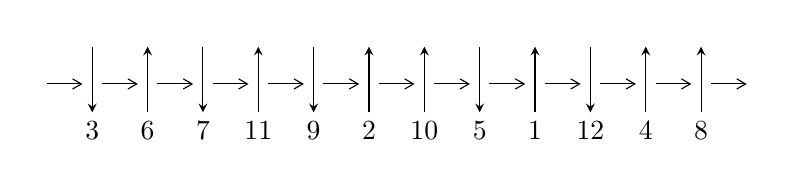
\begin{tikzpicture}[x=20pt, y=17pt]
	% nodes
	\node (C0) at (0, 0) {};
	\node (C1) at (1, 0) {};
	\node (C1U) at (1, +1) {};
	\node (C1D) at (1, -1) {3};

	\node (C2) at (2, 0) {};
	\node (C2U) at (2, +1) {};
	\node (C2D) at (2, -1) {6};

	\node (C3) at (3, 0) {};
	\node (C3U) at (3, +1) {};
	\node (C3D) at (3, -1) {7};

	\node (C4) at (4, 0) {};
	\node (C4U) at (4, +1) {};
	\node (C4D) at (4, -1) {11};

	\node (C5) at (5, 0) {};
	\node (C5U) at (5, +1) {};
	\node (C5D) at (5, -1) {9};

	\node (C6) at (6, 0) {};
	\node (C6U) at (6, +1) {};
	\node (C6D) at (6, -1) {2};

	\node (C7) at (7, 0) {};
	\node (C7U) at (7, +1) {};
	\node (C7D) at (7, -1) {10};

	\node (C8) at (8, 0) {};
	\node (C8U) at (8, +1) {};
	\node (C8D) at (8, -1) {5};

	\node (C9) at (9, 0) {};
	\node (C9U) at (9, +1) {};
	\node (C9D) at (9, -1) {1};

	\node (C10) at (10, 0) {};
	\node (C10U) at (10, +1) {};
	\node (C10D) at (10, -1) {12};

	\node (C11) at (11, 0) {};
	\node (C11U) at (11, +1) {};
	\node (C11D) at (11, -1) {4};

	\node (C12) at (12, 0) {};
	\node (C12U) at (12, +1) {};
	\node (C12D) at (12, -1) {8};
	\node (C13) at (13, 0) {};

	% arrows
	\draw[->,>={angle 60}]
	(C0) edge (C1) (C1) edge (C2) (C2) edge (C3) (C3) edge (C4) (C4) edge (C5) (C5) edge (C6) (C6) edge (C7) (C7) edge (C8) (C8) edge (C9) (C9) edge (C10) (C10) edge (C11) (C11) edge (C12) (C12) edge (C13) ;	\draw[->,>=stealth]
	(C1U) edge (C1D) (C2D) edge (C2U) (C3U) edge (C3D) (C4D) edge (C4U) (C5U) edge (C5D) (C6D) edge (C6U) (C7D) edge (C7U) (C8U) edge (C8D) (C9D) edge (C9U) (C10U) edge (C10D) (C11D) edge (C11U) (C12D) edge (C12U) ;
	\end{tikzpicture} \\
\hhline{~~} \\& 
\textbf{Solving Sequence} \\ \cline{2-2} 
 &
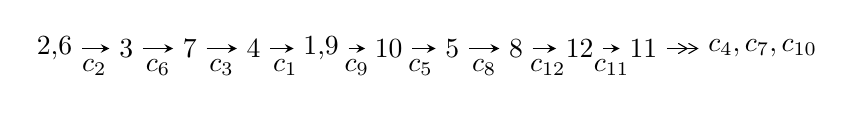
\begin{tikzpicture}[x=23pt, y=7pt]
	% node
	\node (A0) at (-1/8, 0) {2,6};
	\node (A1) at (1, 0) {3};
	\node (A2) at (2, 0) {7};
	\node (A3) at (3, 0) {4};
	\node (A4) at (65/16, 0) {1,9};
	\node (A5) at (41/8, 0) {10};
	\node (A6) at (49/8, 0) {5};
	\node (A7) at (57/8, 0) {8};
	\node (A8) at (65/8, 0) {12};
	\node (A9) at (73/8, 0) {11};
	\node (C1) at (1/2, -1) {$c_{2}$};
	\node (C2) at (3/2, -1) {$c_{6}$};
	\node (C3) at (5/2, -1) {$c_{3}$};
	\node (C4) at (7/2, -1) {$c_{1}$};
	\node (C5) at (37/8, -1) {$c_{9}$};
	\node (C6) at (45/8, -1) {$c_{5}$};
	\node (C7) at (53/8, -1) {$c_{8}$};
	\node (C8) at (61/8, -1) {$c_{12}$};
	\node (C9) at (69/8, -1) {$c_{11}$};
	\node (A10) at (11, 0) {$c_{4},c_{7},c_{10}$};

	% edge
	\draw[->,>=stealth]	
	(A0) edge (A1) (A1) edge (A2) (A2) edge (A3) (A3) edge (A4) (A4) edge (A5) (A5) edge (A6) (A6) edge (A7) (A7) edge (A8) (A8) edge (A9) ;
	\draw[->>,>={angle 60}]	
	(A9) edge (A10);
\end{tikzpicture} \\ 

\end{tabular} \\

\footnotetext{
The image of knot diagram is generated by the software ``\textbf{Draw programme}" developed by Andrew Bartholomew(\url{http://www.layer8.co.uk/maths/draw/index.htm\#Running-draw}), where we modified some parts for our purpose(\url{https://github.com/CATsTAILs/LinksPainter}).
}\phantom \\ \newline 
\centering \textbf{Ideals for irreducible components\footnotemark of $X_{\text{par}}$} 
 
\begin{align*}
I^u_{1}&=\langle 
-8.93536\times10^{235} u^{147}+2.60233\times10^{236} u^{146}+\cdots+1.61998\times10^{236} b-4.36700\times10^{235},\\
\phantom{I^u_{1}}&\phantom{= \langle  }-5.05436\times10^{236} u^{147}+9.67804\times10^{236} u^{146}+\cdots+1.61998\times10^{236} a-1.50588\times10^{236},\\
\phantom{I^u_{1}}&\phantom{= \langle  }u^{148}-2 u^{147}+\cdots- u+1\rangle \\
I^u_{2}&=\langle 
-2 u^{27}- u^{26}+\cdots+b-1,\;- u^{27}+2 u^{26}+\cdots+a+2,\;u^{28}- u^{27}+\cdots- u+1\rangle \\
\\
\end{align*}
\raggedright * 2 irreducible components of $\dim_{\mathbb{C}}=0$, with total 176 representations.\\
\footnotetext{All coefficients of polynomials are rational numbers. But the coefficients are sometimes approximated in decimal forms when there is not enough margin.}
\newpage
\renewcommand{\arraystretch}{1}
\centering \section*{I. $I^u_{1}= \langle -8.94\times10^{235} u^{147}+2.60\times10^{236} u^{146}+\cdots+1.62\times10^{236} b-4.37\times10^{235},\;-5.05\times10^{236} u^{147}+9.68\times10^{236} u^{146}+\cdots+1.62\times10^{236} a-1.51\times10^{236},\;u^{148}-2 u^{147}+\cdots- u+1 \rangle$}
\flushleft \textbf{(i) Arc colorings}\\
\begin{tabular}{m{7pt} m{180pt} m{7pt} m{180pt} }
\flushright $a_{2}=$&$\begin{pmatrix}1\\0\end{pmatrix}$ \\
\flushright $a_{6}=$&$\begin{pmatrix}0\\u\end{pmatrix}$ \\
\flushright $a_{3}=$&$\begin{pmatrix}1\\- u^2\end{pmatrix}$ \\
\flushright $a_{7}=$&$\begin{pmatrix}u\\u\end{pmatrix}$ \\
\flushright $a_{4}=$&$\begin{pmatrix}u^4+u^2+1\\u^4\end{pmatrix}$ \\
\flushright $a_{1}=$&$\begin{pmatrix}u^2+1\\- u^4\end{pmatrix}$ \\
\flushright $a_{9}=$&$\begin{pmatrix}3.12001 u^{147}-5.97417 u^{146}+\cdots+5.16617 u+0.929564\\0.551572 u^{147}-1.60639 u^{146}+\cdots+6.60221 u+0.269571\end{pmatrix}$ \\
\flushright $a_{10}=$&$\begin{pmatrix}4.90742 u^{147}-9.88405 u^{146}+\cdots+10.2567 u+2.03757\\2.74186 u^{147}-5.25117 u^{146}+\cdots+8.07769 u-0.659708\end{pmatrix}$ \\
\flushright $a_{5}=$&$\begin{pmatrix}-3.44700 u^{147}+7.67545 u^{146}+\cdots-9.69461 u-4.30138\\0.766780 u^{147}-0.0367417 u^{146}+\cdots-4.96169 u+0.0605707\end{pmatrix}$ \\
\flushright $a_{8}=$&$\begin{pmatrix}-8.83933 u^{147}+17.8206 u^{146}+\cdots-16.2453 u-4.37980\\-5.65335 u^{147}+10.1649 u^{146}+\cdots-8.27590 u+3.13104\end{pmatrix}$ \\
\flushright $a_{12}=$&$\begin{pmatrix}1.17140 u^{147}-3.95676 u^{146}+\cdots+19.3209 u-11.3326\\-3.30282 u^{147}+6.39633 u^{146}+\cdots+3.20990 u-0.536014\end{pmatrix}$ \\
\flushright $a_{11}=$&$\begin{pmatrix}0.0723142 u^{147}-1.55046 u^{146}+\cdots+13.5943 u-10.7505\\-5.50146 u^{147}+9.54017 u^{146}+\cdots+1.68224 u+0.127919\end{pmatrix}$\\&\end{tabular}
\flushleft \textbf{(ii) Obstruction class $= -1$}\\~\\
\flushleft \textbf{(iii) Cusp Shapes $= 1.08525 u^{147}+1.56569 u^{146}+\cdots+11.7001 u+5.09065$}\\~\\
\newpage\renewcommand{\arraystretch}{1}
\flushleft \textbf{(iv) u-Polynomials at the component}\newline \\
\begin{tabular}{m{50pt}|m{274pt}}
Crossings & \hspace{64pt}u-Polynomials at each crossing \\
\hline $$\begin{aligned}c_{1}\end{aligned}$$&$\begin{aligned}
&u^{148}+76 u^{147}+\cdots+11 u+1
\end{aligned}$\\
\hline $$\begin{aligned}c_{2},c_{6}\end{aligned}$$&$\begin{aligned}
&u^{148}-2 u^{147}+\cdots- u+1
\end{aligned}$\\
\hline $$\begin{aligned}c_{3}\end{aligned}$$&$\begin{aligned}
&u^{148}+2 u^{147}+\cdots-7627619 u+456713
\end{aligned}$\\
\hline $$\begin{aligned}c_{4},c_{11}\end{aligned}$$&$\begin{aligned}
&u^{148}+34 u^{146}+\cdots+u+1
\end{aligned}$\\
\hline $$\begin{aligned}c_{5},c_{8}\end{aligned}$$&$\begin{aligned}
&u^{148}- u^{147}+\cdots+24734 u+1843
\end{aligned}$\\
\hline $$\begin{aligned}c_{7}\end{aligned}$$&$\begin{aligned}
&u^{148}+23 u^{147}+\cdots+58 u+1
\end{aligned}$\\
\hline $$\begin{aligned}c_{9}\end{aligned}$$&$\begin{aligned}
&u^{148}+13 u^{147}+\cdots+1242562 u+100697
\end{aligned}$\\
\hline $$\begin{aligned}c_{10}\end{aligned}$$&$\begin{aligned}
&u^{148}+68 u^{147}+\cdots+19 u+1
\end{aligned}$\\
\hline $$\begin{aligned}c_{12}\end{aligned}$$&$\begin{aligned}
&u^{148}-3 u^{147}+\cdots+52 u+1
\end{aligned}$\\
\hline
\end{tabular}\\~\\
\newpage\renewcommand{\arraystretch}{1}
\flushleft \textbf{(v) Riley Polynomials at the component}\newline \\
\begin{tabular}{m{50pt}|m{274pt}}
Crossings & \hspace{64pt}Riley Polynomials at each crossing \\
\hline $$\begin{aligned}c_{1}\end{aligned}$$&$\begin{aligned}
&y^{148}-4 y^{147}+\cdots+103 y+1
\end{aligned}$\\
\hline $$\begin{aligned}c_{2},c_{6}\end{aligned}$$&$\begin{aligned}
&y^{148}+76 y^{147}+\cdots+11 y+1
\end{aligned}$\\
\hline $$\begin{aligned}c_{3}\end{aligned}$$&$\begin{aligned}
&y^{148}-84 y^{147}+\cdots-9230611190501 y+208586764369
\end{aligned}$\\
\hline $$\begin{aligned}c_{4},c_{11}\end{aligned}$$&$\begin{aligned}
&y^{148}+68 y^{147}+\cdots+19 y+1
\end{aligned}$\\
\hline $$\begin{aligned}c_{5},c_{8}\end{aligned}$$&$\begin{aligned}
&y^{148}-113 y^{147}+\cdots-509628010 y+3396649
\end{aligned}$\\
\hline $$\begin{aligned}c_{7}\end{aligned}$$&$\begin{aligned}
&y^{148}-5 y^{147}+\cdots-358 y+1
\end{aligned}$\\
\hline $$\begin{aligned}c_{9}\end{aligned}$$&$\begin{aligned}
&y^{148}+35 y^{147}+\cdots+1833695584058 y+10139885809
\end{aligned}$\\
\hline $$\begin{aligned}c_{10}\end{aligned}$$&$\begin{aligned}
&y^{148}+36 y^{147}+\cdots+171 y+1
\end{aligned}$\\
\hline $$\begin{aligned}c_{12}\end{aligned}$$&$\begin{aligned}
&y^{148}+7 y^{147}+\cdots-98 y+1
\end{aligned}$\\
\hline
\end{tabular}\\~\\
\newpage\flushleft \textbf{(vi) Complex Volumes and Cusp Shapes}
$$\begin{array}{c|c|c}  
\text{Solutions to }I^u_{1}& \I (\text{vol} + \sqrt{-1}CS) & \text{Cusp shape}\\
 \hline 
\begin{aligned}
u &= -0.094195 + 0.999336 I \\
a &= \phantom{-}0.328602 + 1.117010 I \\
b &= \phantom{-}0.137573 + 1.237080 I\end{aligned}
 & -3.16447 + 2.18690 I & \phantom{-0.000000 } 0 \\ \hline\begin{aligned}
u &= -0.094195 - 0.999336 I \\
a &= \phantom{-}0.328602 - 1.117010 I \\
b &= \phantom{-}0.137573 - 1.237080 I\end{aligned}
 & -3.16447 - 2.18690 I & \phantom{-0.000000 } 0 \\ \hline\begin{aligned}
u &= \phantom{-}0.978749 + 0.166975 I \\
a &= -1.062100 + 0.222854 I \\
b &= \phantom{-}0.688357 - 0.219779 I\end{aligned}
 & -3.72173 + 1.72799 I & \phantom{-0.000000 } 0 \\ \hline\begin{aligned}
u &= \phantom{-}0.978749 - 0.166975 I \\
a &= -1.062100 - 0.222854 I \\
b &= \phantom{-}0.688357 + 0.219779 I\end{aligned}
 & -3.72173 - 1.72799 I & \phantom{-0.000000 } 0 \\ \hline\begin{aligned}
u &= \phantom{-}0.975795 + 0.323601 I \\
a &= -1.196330 + 0.307608 I \\
b &= \phantom{-}0.647571 + 0.063171 I\end{aligned}
 & -3.83865 - 4.09059 I & \phantom{-0.000000 } 0 \\ \hline\begin{aligned}
u &= \phantom{-}0.975795 - 0.323601 I \\
a &= -1.196330 - 0.307608 I \\
b &= \phantom{-}0.647571 - 0.063171 I\end{aligned}
 & -3.83865 + 4.09059 I & \phantom{-0.000000 } 0 \\ \hline\begin{aligned}
u &= -0.507310 + 0.823566 I \\
a &= -0.492109 - 1.107460 I \\
b &= -1.46561 - 1.24894 I\end{aligned}
 & -4.54359 - 4.56469 I & \phantom{-0.000000 } 0 \\ \hline\begin{aligned}
u &= -0.507310 - 0.823566 I \\
a &= -0.492109 + 1.107460 I \\
b &= -1.46561 + 1.24894 I\end{aligned}
 & -4.54359 + 4.56469 I & \phantom{-0.000000 } 0 \\ \hline\begin{aligned}
u &= -0.849870 + 0.428582 I \\
a &= \phantom{-}1.272750 + 0.396740 I \\
b &= -0.341656 + 0.132103 I\end{aligned}
 & -2.83362 + 0.78922 I & \phantom{-0.000000 } 0 \\ \hline\begin{aligned}
u &= -0.849870 - 0.428582 I \\
a &= \phantom{-}1.272750 - 0.396740 I \\
b &= -0.341656 - 0.132103 I\end{aligned}
 & -2.83362 - 0.78922 I & \phantom{-0.000000 } 0\\
 \hline 
 \end{array}$$\newpage$$\begin{array}{c|c|c}  
\text{Solutions to }I^u_{1}& \I (\text{vol} + \sqrt{-1}CS) & \text{Cusp shape}\\
 \hline 
\begin{aligned}
u &= \phantom{-}0.598151 + 0.864715 I \\
a &= \phantom{-}0.372791 + 0.774854 I \\
b &= \phantom{-}0.53248 + 1.50869 I\end{aligned}
 & \phantom{-}2.23245 - 1.64680 I & \phantom{-0.000000 } 0 \\ \hline\begin{aligned}
u &= \phantom{-}0.598151 - 0.864715 I \\
a &= \phantom{-}0.372791 - 0.774854 I \\
b &= \phantom{-}0.53248 - 1.50869 I\end{aligned}
 & \phantom{-}2.23245 + 1.64680 I & \phantom{-0.000000 } 0 \\ \hline\begin{aligned}
u &= -0.230852 + 1.041610 I \\
a &= -0.051708 + 0.534460 I \\
b &= -0.390975 + 0.018729 I\end{aligned}
 & -3.72477 + 1.28933 I & \phantom{-0.000000 } 0 \\ \hline\begin{aligned}
u &= -0.230852 - 1.041610 I \\
a &= -0.051708 - 0.534460 I \\
b &= -0.390975 - 0.018729 I\end{aligned}
 & -3.72477 - 1.28933 I & \phantom{-0.000000 } 0 \\ \hline\begin{aligned}
u &= \phantom{-}0.614295 + 0.699956 I \\
a &= \phantom{-}0.995978 + 0.461045 I \\
b &= -0.204773 + 0.104363 I\end{aligned}
 & \phantom{-}2.70556 + 6.39419 I & \phantom{-0.000000 } 0 \\ \hline\begin{aligned}
u &= \phantom{-}0.614295 - 0.699956 I \\
a &= \phantom{-}0.995978 - 0.461045 I \\
b &= -0.204773 - 0.104363 I\end{aligned}
 & \phantom{-}2.70556 - 6.39419 I & \phantom{-0.000000 } 0 \\ \hline\begin{aligned}
u &= \phantom{-}0.705243 + 0.804106 I \\
a &= \phantom{-}0.355815 - 1.028880 I \\
b &= \phantom{-}0.442914 - 1.019280 I\end{aligned}
 & \phantom{-}1.67100 + 6.12333 I & \phantom{-0.000000 } 0 \\ \hline\begin{aligned}
u &= \phantom{-}0.705243 - 0.804106 I \\
a &= \phantom{-}0.355815 + 1.028880 I \\
b &= \phantom{-}0.442914 + 1.019280 I\end{aligned}
 & \phantom{-}1.67100 - 6.12333 I & \phantom{-0.000000 } 0 \\ \hline\begin{aligned}
u &= -0.302256 + 0.876460 I \\
a &= \phantom{-}0.038881 + 0.179502 I \\
b &= \phantom{-}1.33544 + 1.59186 I\end{aligned}
 & \phantom{-}0.94391 - 1.34144 I & \phantom{-0.000000 } 0 \\ \hline\begin{aligned}
u &= -0.302256 - 0.876460 I \\
a &= \phantom{-}0.038881 - 0.179502 I \\
b &= \phantom{-}1.33544 - 1.59186 I\end{aligned}
 & \phantom{-}0.94391 + 1.34144 I & \phantom{-0.000000 } 0\\
 \hline 
 \end{array}$$\newpage$$\begin{array}{c|c|c}  
\text{Solutions to }I^u_{1}& \I (\text{vol} + \sqrt{-1}CS) & \text{Cusp shape}\\
 \hline 
\begin{aligned}
u &= \phantom{-}0.457920 + 0.801622 I \\
a &= \phantom{-}0.568224 + 0.576181 I \\
b &= -0.150439 + 0.781837 I\end{aligned}
 & \phantom{-}0.05173 + 1.90170 I & \phantom{-0.000000 } 0 \\ \hline\begin{aligned}
u &= \phantom{-}0.457920 - 0.801622 I \\
a &= \phantom{-}0.568224 - 0.576181 I \\
b &= -0.150439 - 0.781837 I\end{aligned}
 & \phantom{-}0.05173 - 1.90170 I & \phantom{-0.000000 } 0 \\ \hline\begin{aligned}
u &= -0.551452 + 0.925329 I \\
a &= -0.217913 + 0.770096 I \\
b &= -0.32932 + 1.93065 I\end{aligned}
 & \phantom{-}2.92622 - 2.93528 I & \phantom{-0.000000 } 0 \\ \hline\begin{aligned}
u &= -0.551452 - 0.925329 I \\
a &= -0.217913 - 0.770096 I \\
b &= -0.32932 - 1.93065 I\end{aligned}
 & \phantom{-}2.92622 + 2.93528 I & \phantom{-0.000000 } 0 \\ \hline\begin{aligned}
u &= \phantom{-}0.729923 + 0.799401 I \\
a &= -0.834437 + 0.472703 I \\
b &= -0.406020 + 0.328911 I\end{aligned}
 & \phantom{-}1.70561 - 0.73296 I & \phantom{-0.000000 } 0 \\ \hline\begin{aligned}
u &= \phantom{-}0.729923 - 0.799401 I \\
a &= -0.834437 - 0.472703 I \\
b &= -0.406020 - 0.328911 I\end{aligned}
 & \phantom{-}1.70561 + 0.73296 I & \phantom{-0.000000 } 0 \\ \hline\begin{aligned}
u &= \phantom{-}0.877976 + 0.242939 I \\
a &= \phantom{-}1.65181 + 0.19080 I \\
b &= -0.723758 + 0.321601 I\end{aligned}
 & -3.7523 - 14.2406 I & \phantom{-0.000000 } 0 \\ \hline\begin{aligned}
u &= \phantom{-}0.877976 - 0.242939 I \\
a &= \phantom{-}1.65181 - 0.19080 I \\
b &= -0.723758 - 0.321601 I\end{aligned}
 & -3.7523 + 14.2406 I & \phantom{-0.000000 } 0 \\ \hline\begin{aligned}
u &= -0.412626 + 1.022700 I \\
a &= \phantom{-}0.791782 + 0.699635 I \\
b &= -0.367077 + 0.591343 I\end{aligned}
 & -2.37666 + 1.92149 I & \phantom{-0.000000 } 0 \\ \hline\begin{aligned}
u &= -0.412626 - 1.022700 I \\
a &= \phantom{-}0.791782 - 0.699635 I \\
b &= -0.367077 - 0.591343 I\end{aligned}
 & -2.37666 - 1.92149 I & \phantom{-0.000000 } 0\\
 \hline 
 \end{array}$$\newpage$$\begin{array}{c|c|c}  
\text{Solutions to }I^u_{1}& \I (\text{vol} + \sqrt{-1}CS) & \text{Cusp shape}\\
 \hline 
\begin{aligned}
u &= -0.803777 + 0.761287 I \\
a &= \phantom{-}0.942167 + 0.420110 I \\
b &= \phantom{-}0.277599 + 0.467456 I\end{aligned}
 & \phantom{-}0.26947 + 5.93833 I & \phantom{-0.000000 } 0 \\ \hline\begin{aligned}
u &= -0.803777 - 0.761287 I \\
a &= \phantom{-}0.942167 - 0.420110 I \\
b &= \phantom{-}0.277599 - 0.467456 I\end{aligned}
 & \phantom{-}0.26947 - 5.93833 I & \phantom{-0.000000 } 0 \\ \hline\begin{aligned}
u &= -0.845808 + 0.256301 I \\
a &= -1.60157 + 0.15845 I \\
b &= \phantom{-}0.624980 + 0.413153 I\end{aligned}
 & -1.42164 + 8.51643 I & \phantom{-0.000000 } 0 \\ \hline\begin{aligned}
u &= -0.845808 - 0.256301 I \\
a &= -1.60157 - 0.15845 I \\
b &= \phantom{-}0.624980 - 0.413153 I\end{aligned}
 & -1.42164 - 8.51643 I & \phantom{-0.000000 } 0 \\ \hline\begin{aligned}
u &= -0.271784 + 0.829466 I \\
a &= -0.581523 + 1.279840 I \\
b &= \phantom{-}0.952850 + 0.719603 I\end{aligned}
 & -2.40401 - 6.32586 I & \phantom{-0.000000 } 0 \\ \hline\begin{aligned}
u &= -0.271784 - 0.829466 I \\
a &= -0.581523 - 1.279840 I \\
b &= \phantom{-}0.952850 - 0.719603 I\end{aligned}
 & -2.40401 + 6.32586 I & \phantom{-0.000000 } 0 \\ \hline\begin{aligned}
u &= \phantom{-}0.327173 + 0.807475 I \\
a &= \phantom{-}0.416283 + 0.881244 I \\
b &= -0.362159 + 0.639328 I\end{aligned}
 & -0.30820 + 1.83950 I & \phantom{-0.000000 } 0 \\ \hline\begin{aligned}
u &= \phantom{-}0.327173 - 0.807475 I \\
a &= \phantom{-}0.416283 - 0.881244 I \\
b &= -0.362159 - 0.639328 I\end{aligned}
 & -0.30820 - 1.83950 I & \phantom{-0.000000 } 0 \\ \hline\begin{aligned}
u &= -0.732313 + 0.859267 I \\
a &= -0.336296 - 1.067240 I \\
b &= -0.253821 - 1.257030 I\end{aligned}
 & -0.05820 - 11.61000 I & \phantom{-0.000000 } 0 \\ \hline\begin{aligned}
u &= -0.732313 - 0.859267 I \\
a &= -0.336296 + 1.067240 I \\
b &= -0.253821 + 1.257030 I\end{aligned}
 & -0.05820 + 11.61000 I & \phantom{-0.000000 } 0\\
 \hline 
 \end{array}$$\newpage$$\begin{array}{c|c|c}  
\text{Solutions to }I^u_{1}& \I (\text{vol} + \sqrt{-1}CS) & \text{Cusp shape}\\
 \hline 
\begin{aligned}
u &= \phantom{-}0.538512 + 0.994874 I \\
a &= -0.334765 + 0.503156 I \\
b &= -0.832714 - 0.173183 I\end{aligned}
 & \phantom{-}0.40241 + 2.45854 I & \phantom{-0.000000 } 0 \\ \hline\begin{aligned}
u &= \phantom{-}0.538512 - 0.994874 I \\
a &= -0.334765 - 0.503156 I \\
b &= -0.832714 + 0.173183 I\end{aligned}
 & \phantom{-}0.40241 - 2.45854 I & \phantom{-0.000000 } 0 \\ \hline\begin{aligned}
u &= -0.570545 + 0.631994 I \\
a &= -1.025060 + 0.277355 I \\
b &= \phantom{-}0.496332 + 0.064601 I\end{aligned}
 & \phantom{-}3.77932 - 1.54987 I & \phantom{-0.000000 } 0 \\ \hline\begin{aligned}
u &= -0.570545 - 0.631994 I \\
a &= -1.025060 - 0.277355 I \\
b &= \phantom{-}0.496332 - 0.064601 I\end{aligned}
 & \phantom{-}3.77932 + 1.54987 I & \phantom{-0.000000 } 0 \\ \hline\begin{aligned}
u &= \phantom{-}0.350751 + 1.098840 I \\
a &= \phantom{-}0.934047 + 0.146504 I \\
b &= \phantom{-}1.074220 + 0.535335 I\end{aligned}
 & -1.356000 + 0.219520 I & \phantom{-0.000000 } 0 \\ \hline\begin{aligned}
u &= \phantom{-}0.350751 - 1.098840 I \\
a &= \phantom{-}0.934047 - 0.146504 I \\
b &= \phantom{-}1.074220 - 0.535335 I\end{aligned}
 & -1.356000 - 0.219520 I & \phantom{-0.000000 } 0 \\ \hline\begin{aligned}
u &= -0.399311 + 1.082190 I \\
a &= -0.64562 - 1.28019 I \\
b &= -0.39699 - 2.90380 I\end{aligned}
 & -6.47002 - 1.38061 I & \phantom{-0.000000 } 0 \\ \hline\begin{aligned}
u &= -0.399311 - 1.082190 I \\
a &= -0.64562 + 1.28019 I \\
b &= -0.39699 + 2.90380 I\end{aligned}
 & -6.47002 + 1.38061 I & \phantom{-0.000000 } 0 \\ \hline\begin{aligned}
u &= \phantom{-}0.496928 + 1.049490 I \\
a &= \phantom{-}0.414745 + 0.477428 I \\
b &= -0.173860 + 0.655148 I\end{aligned}
 & -0.37344 + 2.64441 I & \phantom{-0.000000 } 0 \\ \hline\begin{aligned}
u &= \phantom{-}0.496928 - 1.049490 I \\
a &= \phantom{-}0.414745 - 0.477428 I \\
b &= -0.173860 - 0.655148 I\end{aligned}
 & -0.37344 - 2.64441 I & \phantom{-0.000000 } 0\\
 \hline 
 \end{array}$$\newpage$$\begin{array}{c|c|c}  
\text{Solutions to }I^u_{1}& \I (\text{vol} + \sqrt{-1}CS) & \text{Cusp shape}\\
 \hline 
\begin{aligned}
u &= -0.829917 + 0.096494 I \\
a &= \phantom{-}0.999880 - 0.166069 I \\
b &= -0.485211 - 0.294425 I\end{aligned}
 & -2.47161 + 1.70417 I & \phantom{-0.000000 } 0. - 3.02001 I \\ \hline\begin{aligned}
u &= -0.829917 - 0.096494 I \\
a &= \phantom{-}0.999880 + 0.166069 I \\
b &= -0.485211 + 0.294425 I\end{aligned}
 & -2.47161 - 1.70417 I & \phantom{-0.000000 -}0. + 3.02001 I \\ \hline\begin{aligned}
u &= \phantom{-}0.458761 + 1.071170 I \\
a &= -0.729221 + 0.248734 I \\
b &= -0.144459 - 0.256168 I\end{aligned}
 & -0.50434 + 4.02422 I & \phantom{-0.000000 } 0 \\ \hline\begin{aligned}
u &= \phantom{-}0.458761 - 1.071170 I \\
a &= -0.729221 - 0.248734 I \\
b &= -0.144459 + 0.256168 I\end{aligned}
 & -0.50434 - 4.02422 I & \phantom{-0.000000 } 0 \\ \hline\begin{aligned}
u &= \phantom{-}0.620790 + 0.547942 I \\
a &= \phantom{-}0.566415 - 0.735155 I \\
b &= \phantom{-}0.867114 + 0.126647 I\end{aligned}
 & \phantom{-}1.70567 + 2.12132 I & \phantom{-}5.97809 - 8.47541 I \\ \hline\begin{aligned}
u &= \phantom{-}0.620790 - 0.547942 I \\
a &= \phantom{-}0.566415 + 0.735155 I \\
b &= \phantom{-}0.867114 - 0.126647 I\end{aligned}
 & \phantom{-}1.70567 - 2.12132 I & \phantom{-}5.97809 + 8.47541 I \\ \hline\begin{aligned}
u &= -0.322175 + 1.128650 I \\
a &= -1.062420 + 0.050724 I \\
b &= -1.59933 + 0.47016 I\end{aligned}
 & -3.32302 + 4.78199 I & \phantom{-0.000000 } 0 \\ \hline\begin{aligned}
u &= -0.322175 - 1.128650 I \\
a &= -1.062420 - 0.050724 I \\
b &= -1.59933 - 0.47016 I\end{aligned}
 & -3.32302 - 4.78199 I & \phantom{-0.000000 } 0 \\ \hline\begin{aligned}
u &= \phantom{-}0.792737 + 0.193318 I \\
a &= \phantom{-}1.65458 + 0.03445 I \\
b &= -0.777965 + 0.685230 I\end{aligned}
 & -7.48672 - 5.32621 I & -3.30327 + 4.49709 I \\ \hline\begin{aligned}
u &= \phantom{-}0.792737 - 0.193318 I \\
a &= \phantom{-}1.65458 - 0.03445 I \\
b &= -0.777965 - 0.685230 I\end{aligned}
 & -7.48672 + 5.32621 I & -3.30327 - 4.49709 I\\
 \hline 
 \end{array}$$\newpage$$\begin{array}{c|c|c}  
\text{Solutions to }I^u_{1}& \I (\text{vol} + \sqrt{-1}CS) & \text{Cusp shape}\\
 \hline 
\begin{aligned}
u &= -0.456979 + 1.100050 I \\
a &= \phantom{-}0.237618 + 0.851844 I \\
b &= \phantom{-}0.18101 + 3.78515 I\end{aligned}
 & -0.81545 - 3.66987 I & \phantom{-0.000000 } 0 \\ \hline\begin{aligned}
u &= -0.456979 - 1.100050 I \\
a &= \phantom{-}0.237618 - 0.851844 I \\
b &= \phantom{-}0.18101 - 3.78515 I\end{aligned}
 & -0.81545 + 3.66987 I & \phantom{-0.000000 } 0 \\ \hline\begin{aligned}
u &= -0.715111 + 0.374405 I \\
a &= -0.195776 - 0.263669 I \\
b &= -0.364634 + 0.389793 I\end{aligned}
 & \phantom{-}0.54126 + 3.54143 I & \phantom{-}3.75434 - 0.34615 I \\ \hline\begin{aligned}
u &= -0.715111 - 0.374405 I \\
a &= -0.195776 + 0.263669 I \\
b &= -0.364634 - 0.389793 I\end{aligned}
 & \phantom{-}0.54126 - 3.54143 I & \phantom{-}3.75434 + 0.34615 I \\ \hline\begin{aligned}
u &= \phantom{-}0.420682 + 1.124150 I \\
a &= -0.330865 + 0.820359 I \\
b &= -1.08154 + 3.92517 I\end{aligned}
 & -4.84937 - 1.82765 I & \phantom{-0.000000 } 0 \\ \hline\begin{aligned}
u &= \phantom{-}0.420682 - 1.124150 I \\
a &= -0.330865 - 0.820359 I \\
b &= -1.08154 - 3.92517 I\end{aligned}
 & -4.84937 + 1.82765 I & \phantom{-0.000000 } 0 \\ \hline\begin{aligned}
u &= \phantom{-}0.594507 + 0.512607 I \\
a &= \phantom{-}0.605447 + 0.286351 I \\
b &= \phantom{-}0.325128 + 0.549340 I\end{aligned}
 & \phantom{-}1.22529 + 1.67906 I & \phantom{-}5.39633 - 3.05067 I \\ \hline\begin{aligned}
u &= \phantom{-}0.594507 - 0.512607 I \\
a &= \phantom{-}0.605447 - 0.286351 I \\
b &= \phantom{-}0.325128 - 0.549340 I\end{aligned}
 & \phantom{-}1.22529 - 1.67906 I & \phantom{-}5.39633 + 3.05067 I \\ \hline\begin{aligned}
u &= \phantom{-}0.450266 + 1.128750 I \\
a &= \phantom{-}0.86257 - 1.22449 I \\
b &= \phantom{-}0.74080 - 3.05187 I\end{aligned}
 & -7.68132 + 5.02347 I & \phantom{-0.000000 } 0 \\ \hline\begin{aligned}
u &= \phantom{-}0.450266 - 1.128750 I \\
a &= \phantom{-}0.86257 + 1.22449 I \\
b &= \phantom{-}0.74080 + 3.05187 I\end{aligned}
 & -7.68132 - 5.02347 I & \phantom{-0.000000 } 0\\
 \hline 
 \end{array}$$\newpage$$\begin{array}{c|c|c}  
\text{Solutions to }I^u_{1}& \I (\text{vol} + \sqrt{-1}CS) & \text{Cusp shape}\\
 \hline 
\begin{aligned}
u &= -0.741244 + 0.254652 I \\
a &= \phantom{-}0.54082 - 1.51334 I \\
b &= \phantom{-}0.005226 - 0.332551 I\end{aligned}
 & \phantom{-}0.74086 + 7.93059 I & \phantom{-}2.74611 - 7.67444 I \\ \hline\begin{aligned}
u &= -0.741244 - 0.254652 I \\
a &= \phantom{-}0.54082 + 1.51334 I \\
b &= \phantom{-}0.005226 + 0.332551 I\end{aligned}
 & \phantom{-}0.74086 - 7.93059 I & \phantom{-}2.74611 + 7.67444 I \\ \hline\begin{aligned}
u &= \phantom{-}0.451263 + 1.131820 I \\
a &= \phantom{-}0.067834 - 1.397070 I \\
b &= \phantom{-}0.71217 - 3.63104 I\end{aligned}
 & -7.67016 + 2.76940 I & \phantom{-0.000000 } 0 \\ \hline\begin{aligned}
u &= \phantom{-}0.451263 - 1.131820 I \\
a &= \phantom{-}0.067834 + 1.397070 I \\
b &= \phantom{-}0.71217 + 3.63104 I\end{aligned}
 & -7.67016 - 2.76940 I & \phantom{-0.000000 } 0 \\ \hline\begin{aligned}
u &= -0.537926 + 1.093450 I \\
a &= -0.053904 + 0.775024 I \\
b &= \phantom{-}1.14332 + 1.50502 I\end{aligned}
 & -1.12518 - 8.59303 I & \phantom{-0.000000 } 0 \\ \hline\begin{aligned}
u &= -0.537926 - 1.093450 I \\
a &= -0.053904 - 0.775024 I \\
b &= \phantom{-}1.14332 - 1.50502 I\end{aligned}
 & -1.12518 + 8.59303 I & \phantom{-0.000000 } 0 \\ \hline\begin{aligned}
u &= \phantom{-}0.477248 + 1.128980 I \\
a &= -0.259172 + 0.945359 I \\
b &= \phantom{-}0.56481 + 3.87576 I\end{aligned}
 & -4.44020 + 9.57309 I & \phantom{-0.000000 } 0 \\ \hline\begin{aligned}
u &= \phantom{-}0.477248 - 1.128980 I \\
a &= -0.259172 - 0.945359 I \\
b &= \phantom{-}0.56481 - 3.87576 I\end{aligned}
 & -4.44020 - 9.57309 I & \phantom{-0.000000 } 0 \\ \hline\begin{aligned}
u &= -0.673692 + 0.371028 I \\
a &= -1.172060 - 0.111708 I \\
b &= -0.149098 + 0.813558 I\end{aligned}
 & \phantom{-}0.98324 + 3.90006 I & \phantom{-}8.23651 - 5.87685 I \\ \hline\begin{aligned}
u &= -0.673692 - 0.371028 I \\
a &= -1.172060 + 0.111708 I \\
b &= -0.149098 - 0.813558 I\end{aligned}
 & \phantom{-}0.98324 - 3.90006 I & \phantom{-}8.23651 + 5.87685 I\\
 \hline 
 \end{array}$$\newpage$$\begin{array}{c|c|c}  
\text{Solutions to }I^u_{1}& \I (\text{vol} + \sqrt{-1}CS) & \text{Cusp shape}\\
 \hline 
\begin{aligned}
u &= -0.407315 + 1.164450 I \\
a &= -0.671591 - 0.200838 I \\
b &= -0.691548 - 0.595255 I\end{aligned}
 & -6.13142 - 2.11386 I & \phantom{-0.000000 } 0 \\ \hline\begin{aligned}
u &= -0.407315 - 1.164450 I \\
a &= -0.671591 + 0.200838 I \\
b &= -0.691548 + 0.595255 I\end{aligned}
 & -6.13142 + 2.11386 I & \phantom{-0.000000 } 0 \\ \hline\begin{aligned}
u &= -0.561749 + 1.102850 I \\
a &= \phantom{-}0.089185 + 0.213451 I \\
b &= \phantom{-}0.853807 + 0.008570 I\end{aligned}
 & -1.59412 - 8.43476 I & \phantom{-0.000000 } 0 \\ \hline\begin{aligned}
u &= -0.561749 - 1.102850 I \\
a &= \phantom{-}0.089185 - 0.213451 I \\
b &= \phantom{-}0.853807 - 0.008570 I\end{aligned}
 & -1.59412 + 8.43476 I & \phantom{-0.000000 } 0 \\ \hline\begin{aligned}
u &= -0.743692 + 0.159366 I \\
a &= \phantom{-}1.58736 - 0.22169 I \\
b &= -0.423945 - 0.252612 I\end{aligned}
 & -2.52813 + 1.53343 I & \phantom{-}0.54596 - 1.85069 I \\ \hline\begin{aligned}
u &= -0.743692 - 0.159366 I \\
a &= \phantom{-}1.58736 + 0.22169 I \\
b &= -0.423945 + 0.252612 I\end{aligned}
 & -2.52813 - 1.53343 I & \phantom{-}0.54596 + 1.85069 I \\ \hline\begin{aligned}
u &= \phantom{-}0.521147 + 1.129620 I \\
a &= -0.927754 - 0.338704 I \\
b &= -1.12919 - 0.87813 I\end{aligned}
 & -0.14290 + 7.42320 I & \phantom{-0.000000 } 0 \\ \hline\begin{aligned}
u &= \phantom{-}0.521147 - 1.129620 I \\
a &= -0.927754 + 0.338704 I \\
b &= -1.12919 + 0.87813 I\end{aligned}
 & -0.14290 - 7.42320 I & \phantom{-0.000000 } 0 \\ \hline\begin{aligned}
u &= -0.744636 + 0.100857 I \\
a &= \phantom{-}0.815304 - 0.726174 I \\
b &= -0.370093 - 0.297368 I\end{aligned}
 & -2.51905 + 1.79037 I & -1.08608 - 3.70094 I \\ \hline\begin{aligned}
u &= -0.744636 - 0.100857 I \\
a &= \phantom{-}0.815304 + 0.726174 I \\
b &= -0.370093 + 0.297368 I\end{aligned}
 & -2.51905 - 1.79037 I & -1.08608 + 3.70094 I\\
 \hline 
 \end{array}$$\newpage$$\begin{array}{c|c|c}  
\text{Solutions to }I^u_{1}& \I (\text{vol} + \sqrt{-1}CS) & \text{Cusp shape}\\
 \hline 
\begin{aligned}
u &= \phantom{-}0.335342 + 1.202770 I \\
a &= -0.542905 + 0.996111 I \\
b &= \phantom{-}0.31098 + 2.76756 I\end{aligned}
 & -11.72300 - 1.63235 I & \phantom{-0.000000 } 0 \\ \hline\begin{aligned}
u &= \phantom{-}0.335342 - 1.202770 I \\
a &= -0.542905 - 0.996111 I \\
b &= \phantom{-}0.31098 - 2.76756 I\end{aligned}
 & -11.72300 + 1.63235 I & \phantom{-0.000000 } 0 \\ \hline\begin{aligned}
u &= -0.333069 + 0.665307 I \\
a &= \phantom{-}0.49623 + 1.56070 I \\
b &= \phantom{-}0.511761 - 0.246982 I\end{aligned}
 & -4.05684 + 0.78238 I & -2.41428 + 1.66037 I \\ \hline\begin{aligned}
u &= -0.333069 - 0.665307 I \\
a &= \phantom{-}0.49623 - 1.56070 I \\
b &= \phantom{-}0.511761 + 0.246982 I\end{aligned}
 & -4.05684 - 0.78238 I & -2.41428 - 1.66037 I \\ \hline\begin{aligned}
u &= -0.274221 + 1.226330 I \\
a &= \phantom{-}0.582922 + 0.982247 I \\
b &= \phantom{-}0.20404 + 2.58454 I\end{aligned}
 & -6.17524 + 4.96683 I & \phantom{-0.000000 } 0 \\ \hline\begin{aligned}
u &= -0.274221 - 1.226330 I \\
a &= \phantom{-}0.582922 - 0.982247 I \\
b &= \phantom{-}0.20404 - 2.58454 I\end{aligned}
 & -6.17524 - 4.96683 I & \phantom{-0.000000 } 0 \\ \hline\begin{aligned}
u &= -0.385278 + 1.196360 I \\
a &= -0.581886 - 0.779805 I \\
b &= -0.48929 - 2.04048 I\end{aligned}
 & -6.47605 - 2.30153 I & \phantom{-0.000000 } 0 \\ \hline\begin{aligned}
u &= -0.385278 - 1.196360 I \\
a &= -0.581886 + 0.779805 I \\
b &= -0.48929 + 2.04048 I\end{aligned}
 & -6.47605 + 2.30153 I & \phantom{-0.000000 } 0 \\ \hline\begin{aligned}
u &= -0.508738 + 1.149490 I \\
a &= -0.053152 - 1.122090 I \\
b &= -0.36993 - 2.95291 I\end{aligned}
 & -5.35931 - 6.18141 I & \phantom{-0.000000 } 0 \\ \hline\begin{aligned}
u &= -0.508738 - 1.149490 I \\
a &= -0.053152 + 1.122090 I \\
b &= -0.36993 + 2.95291 I\end{aligned}
 & -5.35931 + 6.18141 I & \phantom{-0.000000 } 0\\
 \hline 
 \end{array}$$\newpage$$\begin{array}{c|c|c}  
\text{Solutions to }I^u_{1}& \I (\text{vol} + \sqrt{-1}CS) & \text{Cusp shape}\\
 \hline 
\begin{aligned}
u &= -0.320549 + 1.216140 I \\
a &= -0.332873 - 0.934936 I \\
b &= -0.00186 - 2.38927 I\end{aligned}
 & -6.67201 - 2.21444 I & \phantom{-0.000000 } 0 \\ \hline\begin{aligned}
u &= -0.320549 - 1.216140 I \\
a &= -0.332873 + 0.934936 I \\
b &= -0.00186 + 2.38927 I\end{aligned}
 & -6.67201 + 2.21444 I & \phantom{-0.000000 } 0 \\ \hline\begin{aligned}
u &= \phantom{-}0.425964 + 1.185020 I \\
a &= \phantom{-}0.931362 - 0.939815 I \\
b &= \phantom{-}1.18213 - 2.57500 I\end{aligned}
 & -7.89986 - 0.93437 I & \phantom{-0.000000 } 0 \\ \hline\begin{aligned}
u &= \phantom{-}0.425964 - 1.185020 I \\
a &= \phantom{-}0.931362 + 0.939815 I \\
b &= \phantom{-}1.18213 + 2.57500 I\end{aligned}
 & -7.89986 + 0.93437 I & \phantom{-0.000000 } 0 \\ \hline\begin{aligned}
u &= \phantom{-}0.736916 + 0.051206 I \\
a &= -1.94600 - 0.90629 I \\
b &= \phantom{-}0.558879 - 0.288383 I\end{aligned}
 & -4.35838 - 5.05167 I & -3.25940 + 7.90426 I \\ \hline\begin{aligned}
u &= \phantom{-}0.736916 - 0.051206 I \\
a &= -1.94600 + 0.90629 I \\
b &= \phantom{-}0.558879 + 0.288383 I\end{aligned}
 & -4.35838 + 5.05167 I & -3.25940 - 7.90426 I \\ \hline\begin{aligned}
u &= -0.533688 + 1.145760 I \\
a &= \phantom{-}0.986026 - 0.494540 I \\
b &= \phantom{-}1.43242 - 1.08748 I\end{aligned}
 & -1.86160 - 12.74340 I & \phantom{-0.000000 } 0 \\ \hline\begin{aligned}
u &= -0.533688 - 1.145760 I \\
a &= \phantom{-}0.986026 + 0.494540 I \\
b &= \phantom{-}1.43242 + 1.08748 I\end{aligned}
 & -1.86160 + 12.74340 I & \phantom{-0.000000 } 0 \\ \hline\begin{aligned}
u &= -0.464254 + 1.176790 I \\
a &= \phantom{-}0.276099 - 0.367655 I \\
b &= \phantom{-}0.01692 - 1.52073 I\end{aligned}
 & -5.71204 - 6.27548 I & \phantom{-0.000000 } 0 \\ \hline\begin{aligned}
u &= -0.464254 - 1.176790 I \\
a &= \phantom{-}0.276099 + 0.367655 I \\
b &= \phantom{-}0.01692 + 1.52073 I\end{aligned}
 & -5.71204 + 6.27548 I & \phantom{-0.000000 } 0\\
 \hline 
 \end{array}$$\newpage$$\begin{array}{c|c|c}  
\text{Solutions to }I^u_{1}& \I (\text{vol} + \sqrt{-1}CS) & \text{Cusp shape}\\
 \hline 
\begin{aligned}
u &= \phantom{-}0.685527 + 0.260417 I \\
a &= -0.36382 - 1.43194 I \\
b &= \phantom{-}0.062293 - 0.481338 I\end{aligned}
 & \phantom{-}2.36352 - 2.78842 I & \phantom{-}5.99487 + 2.61021 I \\ \hline\begin{aligned}
u &= \phantom{-}0.685527 - 0.260417 I \\
a &= -0.36382 + 1.43194 I \\
b &= \phantom{-}0.062293 + 0.481338 I\end{aligned}
 & \phantom{-}2.36352 + 2.78842 I & \phantom{-}5.99487 - 2.61021 I \\ \hline\begin{aligned}
u &= \phantom{-}0.470524 + 1.178780 I \\
a &= -0.221532 - 1.312780 I \\
b &= -0.21240 - 3.56169 I\end{aligned}
 & -7.58338 + 9.46926 I & \phantom{-0.000000 } 0 \\ \hline\begin{aligned}
u &= \phantom{-}0.470524 - 1.178780 I \\
a &= -0.221532 + 1.312780 I \\
b &= -0.21240 + 3.56169 I\end{aligned}
 & -7.58338 - 9.46926 I & \phantom{-0.000000 } 0 \\ \hline\begin{aligned}
u &= \phantom{-}0.173472 + 1.261970 I \\
a &= \phantom{-}0.119485 - 1.064980 I \\
b &= -0.17683 - 2.82048 I\end{aligned}
 & -9.56750 - 0.58327 I & \phantom{-0.000000 } 0 \\ \hline\begin{aligned}
u &= \phantom{-}0.173472 - 1.261970 I \\
a &= \phantom{-}0.119485 + 1.064980 I \\
b &= -0.17683 + 2.82048 I\end{aligned}
 & -9.56750 + 0.58327 I & \phantom{-0.000000 } 0 \\ \hline\begin{aligned}
u &= -0.052055 + 0.719773 I \\
a &= -0.361204 - 0.861064 I \\
b &= -2.43699 + 0.17170 I\end{aligned}
 & -1.89632 + 4.43860 I & -2.51555 - 2.71424 I \\ \hline\begin{aligned}
u &= -0.052055 - 0.719773 I \\
a &= -0.361204 + 0.861064 I \\
b &= -2.43699 - 0.17170 I\end{aligned}
 & -1.89632 - 4.43860 I & -2.51555 + 2.71424 I \\ \hline\begin{aligned}
u &= -0.574837 + 1.147180 I \\
a &= -0.240883 - 1.033160 I \\
b &= -0.47783 - 2.68338 I\end{aligned}
 & -5.11108 - 6.06792 I & \phantom{-0.000000 } 0 \\ \hline\begin{aligned}
u &= -0.574837 - 1.147180 I \\
a &= -0.240883 + 1.033160 I \\
b &= -0.47783 + 2.68338 I\end{aligned}
 & -5.11108 + 6.06792 I & \phantom{-0.000000 } 0\\
 \hline 
 \end{array}$$\newpage$$\begin{array}{c|c|c}  
\text{Solutions to }I^u_{1}& \I (\text{vol} + \sqrt{-1}CS) & \text{Cusp shape}\\
 \hline 
\begin{aligned}
u &= -0.496998 + 1.187650 I \\
a &= \phantom{-}0.214421 - 0.805894 I \\
b &= \phantom{-}0.15155 - 2.37554 I\end{aligned}
 & -5.68511 - 6.41382 I & \phantom{-0.000000 } 0 \\ \hline\begin{aligned}
u &= -0.496998 - 1.187650 I \\
a &= \phantom{-}0.214421 + 0.805894 I \\
b &= \phantom{-}0.15155 + 2.37554 I\end{aligned}
 & -5.68511 + 6.41382 I & \phantom{-0.000000 } 0 \\ \hline\begin{aligned}
u &= \phantom{-}0.530606 + 1.173690 I \\
a &= -0.136138 + 1.059740 I \\
b &= -1.02384 + 3.38189 I\end{aligned}
 & -10.3635 + 10.2246 I & \phantom{-0.000000 } 0 \\ \hline\begin{aligned}
u &= \phantom{-}0.530606 - 1.173690 I \\
a &= -0.136138 - 1.059740 I \\
b &= -1.02384 - 3.38189 I\end{aligned}
 & -10.3635 - 10.2246 I & \phantom{-0.000000 } 0 \\ \hline\begin{aligned}
u &= \phantom{-}0.281268 + 1.259650 I \\
a &= -0.602164 + 0.997818 I \\
b &= -0.34220 + 2.81243 I\end{aligned}
 & -8.62415 - 10.46360 I & \phantom{-0.000000 } 0 \\ \hline\begin{aligned}
u &= \phantom{-}0.281268 - 1.259650 I \\
a &= -0.602164 - 0.997818 I \\
b &= -0.34220 - 2.81243 I\end{aligned}
 & -8.62415 + 10.46360 I & \phantom{-0.000000 } 0 \\ \hline\begin{aligned}
u &= -0.564926 + 1.177470 I \\
a &= \phantom{-}0.045954 + 1.134820 I \\
b &= \phantom{-}0.50216 + 3.22859 I\end{aligned}
 & -4.1731 - 13.7141 I & \phantom{-0.000000 } 0 \\ \hline\begin{aligned}
u &= -0.564926 - 1.177470 I \\
a &= \phantom{-}0.045954 - 1.134820 I \\
b &= \phantom{-}0.50216 - 3.22859 I\end{aligned}
 & -4.1731 + 13.7141 I & \phantom{-0.000000 } 0 \\ \hline\begin{aligned}
u &= \phantom{-}0.569389 + 1.192980 I \\
a &= -0.064758 + 1.186030 I \\
b &= -0.37213 + 3.42803 I\end{aligned}
 & -6.6088 + 19.5371 I & \phantom{-0.000000 } 0 \\ \hline\begin{aligned}
u &= \phantom{-}0.569389 - 1.192980 I \\
a &= -0.064758 - 1.186030 I \\
b &= -0.37213 - 3.42803 I\end{aligned}
 & -6.6088 - 19.5371 I & \phantom{-0.000000 } 0\\
 \hline 
 \end{array}$$\newpage$$\begin{array}{c|c|c}  
\text{Solutions to }I^u_{1}& \I (\text{vol} + \sqrt{-1}CS) & \text{Cusp shape}\\
 \hline 
\begin{aligned}
u &= -0.347929 + 0.560423 I \\
a &= -0.31115 - 1.70958 I \\
b &= -0.73600 - 2.04863 I\end{aligned}
 & -0.93423 - 5.35665 I & \phantom{-}6.58639 + 7.90798 I \\ \hline\begin{aligned}
u &= -0.347929 - 0.560423 I \\
a &= -0.31115 + 1.70958 I \\
b &= -0.73600 + 2.04863 I\end{aligned}
 & -0.93423 + 5.35665 I & \phantom{-}6.58639 - 7.90798 I \\ \hline\begin{aligned}
u &= \phantom{-}0.307412 + 1.310520 I \\
a &= \phantom{-}0.139548 - 0.884774 I \\
b &= -0.45593 - 2.44833 I\end{aligned}
 & -8.72224 + 6.12567 I & \phantom{-0.000000 } 0 \\ \hline\begin{aligned}
u &= \phantom{-}0.307412 - 1.310520 I \\
a &= \phantom{-}0.139548 + 0.884774 I \\
b &= -0.45593 + 2.44833 I\end{aligned}
 & -8.72224 - 6.12567 I & \phantom{-0.000000 } 0 \\ \hline\begin{aligned}
u &= \phantom{-}0.608156 + 1.207850 I \\
a &= \phantom{-}0.336680 - 0.930581 I \\
b &= \phantom{-}0.47949 - 2.74871 I\end{aligned}
 & -6.60922 + 9.82175 I & \phantom{-0.000000 } 0 \\ \hline\begin{aligned}
u &= \phantom{-}0.608156 - 1.207850 I \\
a &= \phantom{-}0.336680 + 0.930581 I \\
b &= \phantom{-}0.47949 + 2.74871 I\end{aligned}
 & -6.60922 - 9.82175 I & \phantom{-0.000000 } 0 \\ \hline\begin{aligned}
u &= \phantom{-}0.543606 + 1.245390 I \\
a &= \phantom{-}0.273062 - 0.738816 I \\
b &= \phantom{-}0.65790 - 2.53745 I\end{aligned}
 & -7.09036 + 3.70510 I & \phantom{-0.000000 } 0 \\ \hline\begin{aligned}
u &= \phantom{-}0.543606 - 1.245390 I \\
a &= \phantom{-}0.273062 + 0.738816 I \\
b &= \phantom{-}0.65790 + 2.53745 I\end{aligned}
 & -7.09036 - 3.70510 I & \phantom{-0.000000 } 0 \\ \hline\begin{aligned}
u &= \phantom{-}0.574015 + 0.126268 I \\
a &= \phantom{-}1.85452 - 0.05087 I \\
b &= -1.47749 - 0.57039 I\end{aligned}
 & -1.72656 - 5.40426 I & \phantom{-}1.53709 + 7.31225 I \\ \hline\begin{aligned}
u &= \phantom{-}0.574015 - 0.126268 I \\
a &= \phantom{-}1.85452 + 0.05087 I \\
b &= -1.47749 + 0.57039 I\end{aligned}
 & -1.72656 + 5.40426 I & \phantom{-}1.53709 - 7.31225 I\\
 \hline 
 \end{array}$$\newpage$$\begin{array}{c|c|c}  
\text{Solutions to }I^u_{1}& \I (\text{vol} + \sqrt{-1}CS) & \text{Cusp shape}\\
 \hline 
\begin{aligned}
u &= -0.171226 + 0.547986 I \\
a &= \phantom{-}1.02157 + 2.72115 I \\
b &= -0.079412 + 1.148280 I\end{aligned}
 & -4.47220 - 1.61677 I & \phantom{-}0.65648 + 6.33827 I \\ \hline\begin{aligned}
u &= -0.171226 - 0.547986 I \\
a &= \phantom{-}1.02157 - 2.72115 I \\
b &= -0.079412 - 1.148280 I\end{aligned}
 & -4.47220 + 1.61677 I & \phantom{-}0.65648 - 6.33827 I \\ \hline\begin{aligned}
u &= \phantom{-}0.548755 + 0.018675 I \\
a &= -2.93170 - 0.57487 I \\
b &= \phantom{-}0.409304 - 0.558284 I\end{aligned}
 & -4.77059 + 1.15573 I & -3.66714 - 1.69774 I \\ \hline\begin{aligned}
u &= \phantom{-}0.548755 - 0.018675 I \\
a &= -2.93170 + 0.57487 I \\
b &= \phantom{-}0.409304 + 0.558284 I\end{aligned}
 & -4.77059 - 1.15573 I & -3.66714 + 1.69774 I \\ \hline\begin{aligned}
u &= \phantom{-}0.374365 + 0.312762 I \\
a &= \phantom{-}0.37147 - 1.47803 I \\
b &= \phantom{-}0.775279 - 0.881999 I\end{aligned}
 & \phantom{-}1.59458 - 0.23339 I & \phantom{-}8.06627 + 1.34861 I \\ \hline\begin{aligned}
u &= \phantom{-}0.374365 - 0.312762 I \\
a &= \phantom{-}0.37147 + 1.47803 I \\
b &= \phantom{-}0.775279 + 0.881999 I\end{aligned}
 & \phantom{-}1.59458 + 0.23339 I & \phantom{-}8.06627 - 1.34861 I \\ \hline\begin{aligned}
u &= -0.269833 + 0.241695 I \\
a &= -1.78785 - 1.00149 I \\
b &= \phantom{-}1.409520 - 0.107037 I\end{aligned}
 & \phantom{-}1.59970 - 0.04753 I & \phantom{-}6.39277 - 0.92731 I \\ \hline\begin{aligned}
u &= -0.269833 - 0.241695 I \\
a &= -1.78785 + 1.00149 I \\
b &= \phantom{-}1.409520 + 0.107037 I\end{aligned}
 & \phantom{-}1.59970 + 0.04753 I & \phantom{-}6.39277 + 0.92731 I\\
 \hline 
 \end{array}$$\newpage\newpage\renewcommand{\arraystretch}{1}
\centering \section*{II. $I^u_{2}= \langle -2 u^{27}- u^{26}+\cdots+b-1,\;- u^{27}+2 u^{26}+\cdots+a+2,\;u^{28}- u^{27}+\cdots- u+1 \rangle$}
\flushleft \textbf{(i) Arc colorings}\\
\begin{tabular}{m{7pt} m{180pt} m{7pt} m{180pt} }
\flushright $a_{2}=$&$\begin{pmatrix}1\\0\end{pmatrix}$ \\
\flushright $a_{6}=$&$\begin{pmatrix}0\\u\end{pmatrix}$ \\
\flushright $a_{3}=$&$\begin{pmatrix}1\\- u^2\end{pmatrix}$ \\
\flushright $a_{7}=$&$\begin{pmatrix}u\\u\end{pmatrix}$ \\
\flushright $a_{4}=$&$\begin{pmatrix}u^4+u^2+1\\u^4\end{pmatrix}$ \\
\flushright $a_{1}=$&$\begin{pmatrix}u^2+1\\- u^4\end{pmatrix}$ \\
\flushright $a_{9}=$&$\begin{pmatrix}u^{27}-2 u^{26}+\cdots+7 u-2\\2 u^{27}+u^{26}+\cdots+7 u+1\end{pmatrix}$ \\
\flushright $a_{10}=$&$\begin{pmatrix}3 u^{27}-4 u^{26}+\cdots+13 u-4\\2 u^{27}+2 u^{26}+\cdots+6 u+2\end{pmatrix}$ \\
\flushright $a_{5}=$&$\begin{pmatrix}-2 u^{27}+7 u^{26}+\cdots-13 u+7\\u^{27}-4 u^{26}+\cdots-20 u^2-4\end{pmatrix}$ \\
\flushright $a_{8}=$&$\begin{pmatrix}-5 u^{27}+13 u^{26}+\cdots-19 u+13\\4 u^{27}+27 u^{25}+\cdots+7 u+1\end{pmatrix}$ \\
\flushright $a_{12}=$&$\begin{pmatrix}-8 u^{27}+2 u^{26}+\cdots-7 u-9\\-5 u^{27}+6 u^{26}+\cdots-10 u+3\end{pmatrix}$ \\
\flushright $a_{11}=$&$\begin{pmatrix}-7 u^{27}-2 u^{26}+\cdots-2 u-14\\-5 u^{27}+4 u^{26}+\cdots-7 u+1\end{pmatrix}$\\&\end{tabular}
\flushleft \textbf{(ii) Obstruction class $= 1$}\\~\\
\flushleft \textbf{(iii) Cusp Shapes $= -20 u^{27}-2 u^{26}-135 u^{25}-39 u^{24}-443 u^{23}-210 u^{22}-851 u^{21}-616 u^{20}-997 u^{19}-1116 u^{18}-637 u^{17}-1321 u^{16}-157 u^{15}-1001 u^{14}-126 u^{13}-478 u^{12}-497 u^{11}-165 u^{10}-655 u^9-167 u^8-433 u^7-242 u^6-157 u^5-270 u^4-39 u^3-171 u^2-7 u-52$}\\~\\
\newpage\renewcommand{\arraystretch}{1}
\flushleft \textbf{(iv) u-Polynomials at the component}\newline \\
\begin{tabular}{m{50pt}|m{274pt}}
Crossings & \hspace{64pt}u-Polynomials at each crossing \\
\hline $$\begin{aligned}c_{1}\end{aligned}$$&$\begin{aligned}
&u^{28}-15 u^{27}+\cdots-11 u+1
\end{aligned}$\\
\hline $$\begin{aligned}c_{2}\end{aligned}$$&$\begin{aligned}
&u^{28}- u^{27}+\cdots- u+1
\end{aligned}$\\
\hline $$\begin{aligned}c_{3}\end{aligned}$$&$\begin{aligned}
&u^{28}+u^{27}+\cdots+u+1
\end{aligned}$\\
\hline $$\begin{aligned}c_{4}\end{aligned}$$&$\begin{aligned}
&u^{28}+u^{27}+\cdots- u+1
\end{aligned}$\\
\hline $$\begin{aligned}c_{5}\end{aligned}$$&$\begin{aligned}
&u^{28}+2 u^{27}+\cdots-11 u^2+1
\end{aligned}$\\
\hline $$\begin{aligned}c_{6}\end{aligned}$$&$\begin{aligned}
&u^{28}+u^{27}+\cdots+u+1
\end{aligned}$\\
\hline $$\begin{aligned}c_{7}\end{aligned}$$&$\begin{aligned}
&u^{28}-2 u^{27}+\cdots+6 u+1
\end{aligned}$\\
\hline $$\begin{aligned}c_{8}\end{aligned}$$&$\begin{aligned}
&u^{28}-2 u^{27}+\cdots-11 u^2+1
\end{aligned}$\\
\hline $$\begin{aligned}c_{9}\end{aligned}$$&$\begin{aligned}
&u^{28}-2 u^{27}+\cdots-2 u+1
\end{aligned}$\\
\hline $$\begin{aligned}c_{10}\end{aligned}$$&$\begin{aligned}
&u^{28}-15 u^{27}+\cdots-19 u+1
\end{aligned}$\\
\hline $$\begin{aligned}c_{11}\end{aligned}$$&$\begin{aligned}
&u^{28}- u^{27}+\cdots+u+1
\end{aligned}$\\
\hline $$\begin{aligned}c_{12}\end{aligned}$$&$\begin{aligned}
&u^{28}+2 u^{27}+\cdots+2 u+1
\end{aligned}$\\
\hline
\end{tabular}\\~\\
\newpage\renewcommand{\arraystretch}{1}
\flushleft \textbf{(v) Riley Polynomials at the component}\newline \\
\begin{tabular}{m{50pt}|m{274pt}}
Crossings & \hspace{64pt}Riley Polynomials at each crossing \\
\hline $$\begin{aligned}c_{1}\end{aligned}$$&$\begin{aligned}
&y^{28}- y^{27}+\cdots-5 y+1
\end{aligned}$\\
\hline $$\begin{aligned}c_{2},c_{6}\end{aligned}$$&$\begin{aligned}
&y^{28}+15 y^{27}+\cdots+11 y+1
\end{aligned}$\\
\hline $$\begin{aligned}c_{3}\end{aligned}$$&$\begin{aligned}
&y^{28}-17 y^{27}+\cdots+23 y+1
\end{aligned}$\\
\hline $$\begin{aligned}c_{4},c_{11}\end{aligned}$$&$\begin{aligned}
&y^{28}+15 y^{27}+\cdots+19 y+1
\end{aligned}$\\
\hline $$\begin{aligned}c_{5},c_{8}\end{aligned}$$&$\begin{aligned}
&y^{28}-30 y^{27}+\cdots-22 y+1
\end{aligned}$\\
\hline $$\begin{aligned}c_{7}\end{aligned}$$&$\begin{aligned}
&y^{28}-6 y^{27}+\cdots-6 y+1
\end{aligned}$\\
\hline $$\begin{aligned}c_{9}\end{aligned}$$&$\begin{aligned}
&y^{28}-6 y^{27}+\cdots+2 y+1
\end{aligned}$\\
\hline $$\begin{aligned}c_{10}\end{aligned}$$&$\begin{aligned}
&y^{28}+7 y^{27}+\cdots-25 y+1
\end{aligned}$\\
\hline $$\begin{aligned}c_{12}\end{aligned}$$&$\begin{aligned}
&y^{28}+2 y^{27}+\cdots-6 y+1
\end{aligned}$\\
\hline
\end{tabular}\\~\\
\newpage\flushleft \textbf{(vi) Complex Volumes and Cusp Shapes}
$$\begin{array}{c|c|c}  
\text{Solutions to }I^u_{2}& \I (\text{vol} + \sqrt{-1}CS) & \text{Cusp shape}\\
 \hline 
\begin{aligned}
u &= -0.365439 + 0.836410 I \\
a &= -0.387851 + 0.415870 I \\
b &= \phantom{-}0.71789 + 1.58480 I\end{aligned}
 & \phantom{-}1.32260 - 1.60130 I & \phantom{-}8.71562 + 6.45471 I \\ \hline\begin{aligned}
u &= -0.365439 - 0.836410 I \\
a &= -0.387851 - 0.415870 I \\
b &= \phantom{-}0.71789 - 1.58480 I\end{aligned}
 & \phantom{-}1.32260 + 1.60130 I & \phantom{-}8.71562 - 6.45471 I \\ \hline\begin{aligned}
u &= \phantom{-}0.381716 + 1.029330 I \\
a &= \phantom{-}0.648516 - 0.513298 I \\
b &= \phantom{-}0.171375 + 0.757477 I\end{aligned}
 & -3.08626 - 2.62316 I & -1.65800 + 5.02113 I \\ \hline\begin{aligned}
u &= \phantom{-}0.381716 - 1.029330 I \\
a &= \phantom{-}0.648516 + 0.513298 I \\
b &= \phantom{-}0.171375 - 0.757477 I\end{aligned}
 & -3.08626 + 2.62316 I & -1.65800 - 5.02113 I \\ \hline\begin{aligned}
u &= \phantom{-}0.856236 + 0.280811 I \\
a &= -1.387960 + 0.082806 I \\
b &= \phantom{-}0.388646 + 0.076668 I\end{aligned}
 & -3.10049 - 0.21509 I & -4.06964 - 3.93322 I \\ \hline\begin{aligned}
u &= \phantom{-}0.856236 - 0.280811 I \\
a &= -1.387960 - 0.082806 I \\
b &= \phantom{-}0.388646 - 0.076668 I\end{aligned}
 & -3.10049 + 0.21509 I & -4.06964 + 3.93322 I \\ \hline\begin{aligned}
u &= -0.486112 + 0.995622 I \\
a &= -0.203990 - 0.411822 I \\
b &= -0.240558 + 0.877728 I\end{aligned}
 & \phantom{-}0.80932 - 2.87184 I & \phantom{-}9.73391 + 6.16296 I \\ \hline\begin{aligned}
u &= -0.486112 - 0.995622 I \\
a &= -0.203990 + 0.411822 I \\
b &= -0.240558 - 0.877728 I\end{aligned}
 & \phantom{-}0.80932 + 2.87184 I & \phantom{-}9.73391 - 6.16296 I \\ \hline\begin{aligned}
u &= -0.863022 + 0.165510 I \\
a &= \phantom{-}1.47605 + 0.06126 I \\
b &= -0.683724 - 0.004069 I\end{aligned}
 & -3.74191 + 3.30686 I & -2.33673 - 2.10493 I \\ \hline\begin{aligned}
u &= -0.863022 - 0.165510 I \\
a &= \phantom{-}1.47605 - 0.06126 I \\
b &= -0.683724 + 0.004069 I\end{aligned}
 & -3.74191 - 3.30686 I & -2.33673 + 2.10493 I\\
 \hline 
 \end{array}$$\newpage$$\begin{array}{c|c|c}  
\text{Solutions to }I^u_{2}& \I (\text{vol} + \sqrt{-1}CS) & \text{Cusp shape}\\
 \hline 
\begin{aligned}
u &= -0.490056 + 0.670198 I \\
a &= \phantom{-}0.417868 + 0.499022 I \\
b &= \phantom{-}1.194550 + 0.667265 I\end{aligned}
 & \phantom{-}1.89003 - 1.13368 I & \phantom{-}6.62059 + 3.29252 I \\ \hline\begin{aligned}
u &= -0.490056 - 0.670198 I \\
a &= \phantom{-}0.417868 - 0.499022 I \\
b &= \phantom{-}1.194550 - 0.667265 I\end{aligned}
 & \phantom{-}1.89003 + 1.13368 I & \phantom{-}6.62059 - 3.29252 I \\ \hline\begin{aligned}
u &= \phantom{-}0.649260 + 0.516295 I \\
a &= -0.978264 + 0.324319 I \\
b &= -0.747966 + 0.047309 I\end{aligned}
 & -0.10406 - 4.45468 I & \phantom{-}0.81082 + 4.92455 I \\ \hline\begin{aligned}
u &= \phantom{-}0.649260 - 0.516295 I \\
a &= -0.978264 - 0.324319 I \\
b &= -0.747966 - 0.047309 I\end{aligned}
 & -0.10406 + 4.45468 I & \phantom{-}0.81082 - 4.92455 I \\ \hline\begin{aligned}
u &= \phantom{-}0.549710 + 1.067170 I \\
a &= \phantom{-}0.025082 - 0.662017 I \\
b &= \phantom{-}0.681133 - 0.440731 I\end{aligned}
 & -1.81915 + 9.16310 I & -2.52839 - 13.26466 I \\ \hline\begin{aligned}
u &= \phantom{-}0.549710 - 1.067170 I \\
a &= \phantom{-}0.025082 + 0.662017 I \\
b &= \phantom{-}0.681133 + 0.440731 I\end{aligned}
 & -1.81915 - 9.16310 I & -2.52839 + 13.26466 I \\ \hline\begin{aligned}
u &= \phantom{-}0.348454 + 1.149410 I \\
a &= \phantom{-}0.658802 - 1.099010 I \\
b &= \phantom{-}0.92388 - 2.48074 I\end{aligned}
 & -7.39860 + 3.04531 I & -8.09341 - 4.44196 I \\ \hline\begin{aligned}
u &= \phantom{-}0.348454 - 1.149410 I \\
a &= \phantom{-}0.658802 + 1.099010 I \\
b &= \phantom{-}0.92388 + 2.48074 I\end{aligned}
 & -7.39860 - 3.04531 I & -8.09341 + 4.44196 I \\ \hline\begin{aligned}
u &= -0.374671 + 1.175130 I \\
a &= -0.512726 - 1.137850 I \\
b &= -0.50975 - 3.13448 I\end{aligned}
 & -7.86845 - 0.47406 I & -6.80610 + 0.20183 I \\ \hline\begin{aligned}
u &= -0.374671 - 1.175130 I \\
a &= -0.512726 + 1.137850 I \\
b &= -0.50975 + 3.13448 I\end{aligned}
 & -7.86845 + 0.47406 I & -6.80610 - 0.20183 I\\
 \hline 
 \end{array}$$\newpage$$\begin{array}{c|c|c}  
\text{Solutions to }I^u_{2}& \I (\text{vol} + \sqrt{-1}CS) & \text{Cusp shape}\\
 \hline 
\begin{aligned}
u &= \phantom{-}0.227894 + 0.712348 I \\
a &= \phantom{-}0.248942 + 1.342120 I \\
b &= -1.77286 + 1.79816 I\end{aligned}
 & -1.75291 + 5.42762 I & -1.77047 - 8.41574 I \\ \hline\begin{aligned}
u &= \phantom{-}0.227894 - 0.712348 I \\
a &= \phantom{-}0.248942 - 1.342120 I \\
b &= -1.77286 - 1.79816 I\end{aligned}
 & -1.75291 - 5.42762 I & -1.77047 + 8.41574 I \\ \hline\begin{aligned}
u &= \phantom{-}0.023362 + 0.732048 I \\
a &= \phantom{-}0.09845 + 2.19590 I \\
b &= -0.476032 + 0.772669 I\end{aligned}
 & -5.01732 - 1.24897 I & -11.27715 - 0.05900 I \\ \hline\begin{aligned}
u &= \phantom{-}0.023362 - 0.732048 I \\
a &= \phantom{-}0.09845 - 2.19590 I \\
b &= -0.476032 - 0.772669 I\end{aligned}
 & -5.01732 + 1.24897 I & -11.27715 + 0.05900 I \\ \hline\begin{aligned}
u &= -0.496859 + 1.198450 I \\
a &= -0.124720 - 1.049440 I \\
b &= -0.13620 - 3.21782 I\end{aligned}
 & -6.95419 - 8.20241 I & -4.76290 + 6.44782 I \\ \hline\begin{aligned}
u &= -0.496859 - 1.198450 I \\
a &= -0.124720 + 1.049440 I \\
b &= -0.13620 + 3.21782 I\end{aligned}
 & -6.95419 + 8.20241 I & -4.76290 - 6.44782 I \\ \hline\begin{aligned}
u &= \phantom{-}0.539527 + 1.190270 I \\
a &= \phantom{-}0.021804 - 0.999223 I \\
b &= -0.01038 - 2.64689 I\end{aligned}
 & -5.94690 + 5.37088 I & -5.57815 - 1.15124 I \\ \hline\begin{aligned}
u &= \phantom{-}0.539527 - 1.190270 I \\
a &= \phantom{-}0.021804 + 0.999223 I \\
b &= -0.01038 + 2.64689 I\end{aligned}
 & -5.94690 - 5.37088 I & -5.57815 + 1.15124 I\\
 \hline 
 \end{array}$$\newpage
\newpage\renewcommand{\arraystretch}{1}
\centering \section*{ III. u-Polynomials}
\begin{tabular}{m{50pt}|m{274pt}}
Crossings & \hspace{64pt}u-Polynomials at each crossing \\
\hline $$\begin{aligned}c_{1}\end{aligned}$$&$\begin{aligned}
&(u^{28}-15 u^{27}+\cdots-11 u+1)(u^{148}+76 u^{147}+\cdots+11 u+1)
\end{aligned}$\\
\hline $$\begin{aligned}c_{2}\end{aligned}$$&$\begin{aligned}
&(u^{28}- u^{27}+\cdots- u+1)(u^{148}-2 u^{147}+\cdots- u+1)
\end{aligned}$\\
\hline $$\begin{aligned}c_{3}\end{aligned}$$&$\begin{aligned}
&(u^{28}+u^{27}+\cdots+u+1)(u^{148}+2 u^{147}+\cdots-7627619 u+456713)
\end{aligned}$\\
\hline $$\begin{aligned}c_{4}\end{aligned}$$&$\begin{aligned}
&(u^{28}+u^{27}+\cdots- u+1)(u^{148}+34 u^{146}+\cdots+u+1)
\end{aligned}$\\
\hline $$\begin{aligned}c_{5}\end{aligned}$$&$\begin{aligned}
&(u^{28}+2 u^{27}+\cdots-11 u^2+1)(u^{148}- u^{147}+\cdots+24734 u+1843)
\end{aligned}$\\
\hline $$\begin{aligned}c_{6}\end{aligned}$$&$\begin{aligned}
&(u^{28}+u^{27}+\cdots+u+1)(u^{148}-2 u^{147}+\cdots- u+1)
\end{aligned}$\\
\hline $$\begin{aligned}c_{7}\end{aligned}$$&$\begin{aligned}
&(u^{28}-2 u^{27}+\cdots+6 u+1)(u^{148}+23 u^{147}+\cdots+58 u+1)
\end{aligned}$\\
\hline $$\begin{aligned}c_{8}\end{aligned}$$&$\begin{aligned}
&(u^{28}-2 u^{27}+\cdots-11 u^2+1)(u^{148}- u^{147}+\cdots+24734 u+1843)
\end{aligned}$\\
\hline $$\begin{aligned}c_{9}\end{aligned}$$&$\begin{aligned}
&(u^{28}-2 u^{27}+\cdots-2 u+1)(u^{148}+13 u^{147}+\cdots+1242562 u+100697)
\end{aligned}$\\
\hline $$\begin{aligned}c_{10}\end{aligned}$$&$\begin{aligned}
&(u^{28}-15 u^{27}+\cdots-19 u+1)(u^{148}+68 u^{147}+\cdots+19 u+1)
\end{aligned}$\\
\hline $$\begin{aligned}c_{11}\end{aligned}$$&$\begin{aligned}
&(u^{28}- u^{27}+\cdots+u+1)(u^{148}+34 u^{146}+\cdots+u+1)
\end{aligned}$\\
\hline $$\begin{aligned}c_{12}\end{aligned}$$&$\begin{aligned}
&(u^{28}+2 u^{27}+\cdots+2 u+1)(u^{148}-3 u^{147}+\cdots+52 u+1)
\end{aligned}$\\
\hline
\end{tabular}\newpage\renewcommand{\arraystretch}{1}
\centering \section*{ IV. Riley Polynomials}
\begin{tabular}{m{50pt}|m{274pt}}
Crossings & \hspace{64pt}Riley Polynomials at each crossing \\
\hline $$\begin{aligned}c_{1}\end{aligned}$$&$\begin{aligned}
&(y^{28}- y^{27}+\cdots-5 y+1)(y^{148}-4 y^{147}+\cdots+103 y+1)
\end{aligned}$\\
\hline $$\begin{aligned}c_{2},c_{6}\end{aligned}$$&$\begin{aligned}
&(y^{28}+15 y^{27}+\cdots+11 y+1)(y^{148}+76 y^{147}+\cdots+11 y+1)
\end{aligned}$\\
\hline $$\begin{aligned}c_{3}\end{aligned}$$&$\begin{aligned}
&(y^{28}-17 y^{27}+\cdots+23 y+1)\\
&\cdot(y^{148}-84 y^{147}+\cdots-9230611190501 y+208586764369)
\end{aligned}$\\
\hline $$\begin{aligned}c_{4},c_{11}\end{aligned}$$&$\begin{aligned}
&(y^{28}+15 y^{27}+\cdots+19 y+1)(y^{148}+68 y^{147}+\cdots+19 y+1)
\end{aligned}$\\
\hline $$\begin{aligned}c_{5},c_{8}\end{aligned}$$&$\begin{aligned}
&(y^{28}-30 y^{27}+\cdots-22 y+1)\\
&\cdot(y^{148}-113 y^{147}+\cdots-509628010 y+3396649)
\end{aligned}$\\
\hline $$\begin{aligned}c_{7}\end{aligned}$$&$\begin{aligned}
&(y^{28}-6 y^{27}+\cdots-6 y+1)(y^{148}-5 y^{147}+\cdots-358 y+1)
\end{aligned}$\\
\hline $$\begin{aligned}c_{9}\end{aligned}$$&$\begin{aligned}
&(y^{28}-6 y^{27}+\cdots+2 y+1)\\
&\cdot(y^{148}+35 y^{147}+\cdots+1833695584058 y+10139885809)
\end{aligned}$\\
\hline $$\begin{aligned}c_{10}\end{aligned}$$&$\begin{aligned}
&(y^{28}+7 y^{27}+\cdots-25 y+1)(y^{148}+36 y^{147}+\cdots+171 y+1)
\end{aligned}$\\
\hline $$\begin{aligned}c_{12}\end{aligned}$$&$\begin{aligned}
&(y^{28}+2 y^{27}+\cdots-6 y+1)(y^{148}+7 y^{147}+\cdots-98 y+1)
\end{aligned}$\\
\hline
\end{tabular}
\vskip 2pc
\end{document}